\documentclass[
%  printversion,
  biblatex,
  glossaries,
  index
]{kidiplom}

%% Uživatelské příkazy
\newcommand{\pic}[4]{
\begin{figure}[h]
\centering
\includegraphics[width=#1]{#2}
\caption{#3}
\label{fig:#4}
\end{figure}}

%% Název práce, česky a anglicky.
\title{Grafické uživatelské rozhraní pro systém správy verzí Git}
\title[english]{Graphical user interface for version control system Git}

%% Jméno autora práce.
\author{Jaroslav Večeřa}

%% Jméno vedoucího práce (včetně titulů).
\supervisor{Mgr. Radek Janoštík}

%% Anotace práce, včetně anglické
\annotation{Grafické rozhraní pro Windows, které zprostředková přehlednou a intuitivní práci se základními funkcemi systému Git, a to převážně pomocí grafu.}

\annotation[english]{Windows graphical user interface that allows
intuitive git workflow using graph representation.}

%% Klíčová slova práce, včetně anglických. Oddělená (obvykle) středníkem.
\keywords{git; verzování; graf; grafické rozhraní}
\keywords[english]{git; version control; graphical interface}

%% Poděkování
\thanks{Děkuji, děkuji, děkuji.}

%% Cesta k souboru s bibliografií pro její sazbu pomocí BibLaTeXu
\bibliography{bibliografie.bib}

%% Další dodatečné styly (balíky) potřebné pro sazbu vlastního textu
%% práce.
\usepackage{lipsum}
\usepackage{caption}
\usepackage{subcaption}

%% Cesta ke složce s grafikou
\graphicspath{{graphics/}}

%% Reference BibLaTeXu
\bibliography{bibliografie.bib}

\begin{document}
\maketitle

%% Vlastní text závěrečné práce. Pro povinné závěry, před přílohami,
%% použijte prostředí kiconclusions. Povinná je i příloha s obsahem
%% přiloženého CD/DVD.

%% -------------------------------------------------------------------

\newcommand{\BibLaTeX}{\textsc{Bib}\LaTeX}

\section{Úvod}
Při vývoji programů, zvláště pak těch netriviálních, je často třeba
dělat změny nebo nové verze. Protože však není možné vytvořit program
bez chyb, objevuje se také potřeba vracet se k libovolným starším
verzím a zakládat na nich nové, či dokonce vyvíjet více verzí zároveň v
případě skupiny lidí. Tato činnost lze samozřejmě provádět ručně,
zabírá to ale čas a zvyšuje riziko chyby. Může dojít ke změně souboru
nebo jeho smazání na špatném místě. Přece jen udržovat si v úložišti
desítky záloh nebo obměn dat a spravovat je ručně vyžaduje podrobný
popis jednotlivých verzí, který časem musí být značně nepřehledný.
Z tohoto důvodu byly vytvořeny takzvané verzovací systémy.

Systém správy verzí (dále SSV) je zpravidla softwarový nástroj,
umožňující spravovat verze projektu částečně automaticky (nebo alespoň
přehledně a jednoduše). Přitom daný projekt nemusí být zdrojovým kódem
v nějakém programovacím jazyce, může se jednat vlastně o libovolná data.
Vracet zpět provedené změny, nebo pracovat ve skupině lidí může být
užitečné například i grafikům, střihačům videí, spisovatelům a podobně.
Systém uchovává jak soubory samotné, tak různé informace související
se správou verzí. To se samozřejmě napříč konkrétními systémy liší,
obvykle je ale k dispozici:
\begin{itemize}
\item Popis změny (ručně zadaný)
\item Čas změny
\item Autor změny a jeho kontaktní údaje
\end{itemize}

Tyto údaje jsou zejména užitečné v případě týmu lidí pracujících na
společném projektu, historicky však nejprve vznikla skupina takzvaných
lokálních SSV.

\subsection{Lokální SSV}
Tyto systémy se soustředily na práci jednotlivce, celý projekt byl 
ukládán na místním disku a nebyl nikde sdílen. Konkrétním zástupcem je 
například RCS (Revision Control System). RCS si uchovává poslední podobu  
daného souboru spolu se zpětnými rozdíly. Aplikací těchto rozdílů (delt) 
na soubor lze rekonstruovat některou jeho předchozí verzi.

Nevýhoda lokálního SSV je, že projekt je umístěn pouze na jednom 
zařízení, a při chybě disku tak hrozí ztráta dat. Další nevýhodou je 
nemožnost projekty pohodlně sdílet po síti.

\subsection{Centralizované SSV}
Centralizované systémy (CSSV)~\cite{otte} jsou historicky dalším vývojovým stupněm SSV. 
Představují opačný extrém k lokálním SSV, na rozdíl od nich totiž 
většinu souborů a práci přesouvají od koncového uživatele na jeden 
společný centrální server, ten je skrze síť dostupný odkudkoliv na světě. Metodu zachycuje obrázek \ref{fig:centralized} \cite{gitreference}.

\pic{10cm}{centralized.png}{Centralizovaný systém správy verzí}{centralized}

Od chvíle, kdy uživatel $A$ udělá na souboru $S$ nějaké změny a nasdílí
je do společné databáze, už žádný další uživatel nemá aktuální
verzi souboru $S$.
Pro obdržení aktuální verze musí svoji kopii každý opět aktualizovat.
V případě, že další uživatel provedl jiné změny na témže souboru,
systém se je pokusí sloučit dohromady. Uživatelé se tedy nemusí starat o 
případy, ve kterých nedojde k závažnému konfliktu. Pokud však uživatel $A$ 
upravil stejný řádek souboru $S$, jako uživatel $B$, ale jinak, je třeba se 
o vyřešení konfliktu postarat ručně výběrem správné verze, případně
spojením obou změn.

Pro snížení počtu konfliktů je v CSSV dostupná funkce větvení. Umožňuje 
vytvářet historii změn s jiný než lineární strukturou. Větvení se častou 
používá pro implementaci ucelené funkcionality programu, nebo pro 
experimentální záležitosti, které nemusejí být po svém ukončení začleněny 
do projektu. Uživatel může pracovat na verzích větve aniž by ovlivňovaly
verze větve jiného uživatele.

Výhodou CSSV je například
šetření místa jednotlivých uživatelů. Ti na svých zařízeních mají fyzickou 
kopii pouze aktuální verze projektu, zbytek historie je uložen na serveru.
To však přináší nemalá rizika v případě výpadku. Pokud uživatel není
schopen připojení k síti, nemůže na projektu pracovat, jelikož veškerá
práce se systémem vyžaduje síťové připojení. Pokud dokonce dojde k
porušení této společné databáze, veškerá historie dat je nenávratně
ztracena, stejně jako v Lokálním SSV se totiž nachází pouze na jednom místě. Drobnou výhodou 
zůstává, že alespoň aktuální verze se nachází na více zařízeních.

\subsection{Distribuované SSV}
Distribuované systémy (DSSV)~\cite{otte} se vyvinuly po centralizovaných a představují 
jakýsi kompromis obou předchozích systémů. DSSV se snaží těžit z výhod obou 
metod. Projekt lze snadno sdílet pomocí sítě. Kromě uživatelů obsahuje 
servery, na kterých se nachází tzv. vzdálené repozitáře. Tyto repozitáře 
plní stejnou funkci jako v CSSV, nejedná se však o jedinou kopii projektu.
Každý uživatel, který s ním pracuje, vlastní úplnou kopii
celé historie. Jednotlivé repozitáře uživatelů a serverů se mezi sebou 		
aktualizují pomocí k tomu určených příkazů. Tyto příkazy se často nazývají
push (pro pokus včlenit změny do zvoleného vzdáleného repozitáře), fetch
(pro stažení dat ze vzdáleného repozitáře) a pull (pro včlenění dat ze 
vzdáleného repozitáře).

\pic{10cm}{distributed.png}{Distribuovaný systém správy verzí}{distributed}

Jak je v obrázku \ref{fig:distributed} \cite{gitreference} naznačeno přerušovaným spojení mezi uživateli A a B, přímé sdílení projektu sice DSSV umožňuje, není však tolik využívané. Mnohem častěji sdílí uživatelé práci se společným serverem, který tak hraje roli jakéhosi pasivního uživatele, se kterým ostatní komunikují.

Příklady takových nástrojů jsou Mercurial, Bazaar, nebo Git, kterého se
tato práce týká.

\section{Git}
Git~\cite{git} je distribuovaný SSV, který na rozdíl od ostatních SSV uchovává historii   takovým způsobem, že většina operací nad soubory je výrazně rychlejší. V článku~\cite{gitreference-history} je popsána historie vzniku Gitu.

Většina verzovacích systémů má uložený soubor a pro každou jeho verzi dopředné, či zpětné rozdíly. Pomocí skládání těchto rozdílů lze znovu zhotovit libovolnou verzi souboru. Hlavní výhoda tohoto přístupu spočívá v ušetřeném místě, oproti ukládání celé kopie se totiž ušetří části, které se mezi jednotlivými verzemi nezměnily. Má to však dopad na rychlost opětovného sestrojení  konkrétních verzí.

Git naproti tomu uchovává pro jednotlivé verze celé kopie (nazývají se snapchoty). Rychlost sestrojení souborů v historii tak není ovlivněna množstvím verzí, které od té doby byly zhotoveny. Git samozřejmě ukládání optimalizuje, a to tak, že pokud nejsou v souboru provedené změny, místo nového snapshotu se uloží odkaz na starý. Celý repozitář také podléhá bezeztrátové kompresi.

Verze projektu také budeme nazývat revize. Každá revize, kromě počáteční, má jeden nebo více předků. Jeden v případě prostého vytvoření další verze, více v případě slévání změn z více verzí (merge). Celá historie se tak dá reprezentovat jako orientovaný, souvislý a acyklický graf s uzly vyjadřujícími revize a hranami vyjadřujícími vztah rodič -- potomek. Vytvořit aplikaci reprezentující tímto způsobem historii vytvořenou gitem je také hlavní cíl této práce.

Jednotlivé větve pak git ukládá vnitřně pouze jako ukazatele na poslední revizi větve. Při vytváření nových verzí se tyto ukazatele posunují na novější commit. Žádná data o tom, v jaké větvi byla revize původně vytvořena, nejsou k dispozici a často se nedají nijak dohledat. Tato informace bude později důležitá při popisu heuristiky rozmístění uzlů v grafu na straně \pageref{subsec:algorithm}

Poté ještě v repozitáři existuje speciální ukazatel HEAD, který ukazuje na větev, či přímo revizi, které jsou aktuálně prohlíženy.

Následující seznam popisuje základní funkce pro práci s Gitem.

\begin{description}
  \item[Commit]  vytvoří novou verzi, přitom se na ni přesune ukazatel větve, na kterou ukazuje HEAD, případně se posune HEAD, pokud ukazuje přímo na revizi.
  \item[Branch] Vytvoří nový ukazatel větve na aktuální verzi.
  \item[Checkout] znovu sestrojí verzi předanou argumentem. Buď formou větve, kdy HEAD začne odkazovat na onu větev, nebo formou revize přímo, potom HEAD odkazuje na revizi a repozitář se nachází v experimentálním módu.
  \item[Stash] v závislosti na argumentu ukládají, aplikují a mažou provedené změny od poslední verze na strukturu zásobníkového charakteru.
  \item[Merge] spojuje vybrané větve do jedné. V případě, že nelze konflikty automaticky vyřešit, je o to uživatel požádán.
  \item[Rebase] oproti merge manipuluje s historií. Přeskládá revize aktuální větve ($B_1$) jako by se od dané větve ($B_2$) oddělovaly až na konci $B_2$.
  \item[Diff] je nástroj pro vytvoření rozdílů v souborech, nebo celých verzích.
  \item[Log] ukazuje strukturu historie.
  \item[Fetch] stáhne historii ze vzdáleného repozitáře.
  \item[Pull] provede fetch a následně merge.
  \item[Push] naopak začlení změny do vzdáleného repozitáře.
\end{description}

\subsection{Základní postupy práce v Gitu}
Git poskytuje velkou volnost ve způsobu správy větví a to jak lokálně~\cite{gitreference-local} , tak v práci se vzdálenými repozitáři~\cite{gitreference-distributed}.

\subsubsection{Postupy větvení}
\paragraph*{Dlouhodobé větve}
Při práci tímto způsobem obvykle repozitář obsahuje větve tří úrovní. První úroveň tvoří hlavní větev (často s názvem {\it master}, nebo {\it main}), která obsahuje pouze dobře otestované revize připravené k publikaci.

Vedle toho bývá k dispozici větev s názvem jako je {\it next}, nebo {\it develop}, která obsahuje méně stabilní kód, který není ucelený, nebo teprve čeká na otestování. Z této větve jsou revize podle potřeby slučovány do hlavní větve.

Poslední úroveň tvoří větve pro jednotlivé funkcionality. Tyto větve slouží k oddělení funkcionalit, které jsou v současné době ve vývoji. Z nich je práce po dokončení slučována do {\it develop} větve.

\paragraph*{Krátkodobé větve}
Tento způsob práce (někdy nazývaný {\it topic branch}) není tak striktní ve způsobu slučování větví. Dovoluje slučování starších větví do novějších i naopak a tím vzniká tendence udržovat větve krátkodobější a s menším počtem revizí.

Dá se říct, že se jedná o odlehčenou verzi metody dlouhodobých větví, která obsahuje pouze nejnižší úroveň stability. Pro tyto vlastnosti je postup vhodný spíše u menších projektů.

\subsubsection{Distribuovaná práce s větvemi}
\paragraph*{Centralizovaný postup}

Tento postup je hojně využíván hlavně pro svoji jednoduchost. Také je vhodný při přechodu z centralizovaného SSV pro jejich podobnost. Centralizovaný postup je vhodný pro týmy, ve kterých nehraje velkou roli hierarchie vývojářů, popřípadě nejsou příliš početné.

Prostředkem pro sdílení projektu je jediný vzdálený repozitář, ze kterého/který přispěvatelé aktualizují. Uživatelé, kteří chtějí na projektu pracovat, provedou operaci merge, či clone. Pokud naopak chtějí svoji práci sdílet do vzdáleného repozitáře, provedou push. V případě, že jiný uživatel mezitím sdílel svoji práci, nemá daný uživatel aktuální verzi a musí nejprve včlenit historii z centrální databáze do své, poté až provést push. Přitom samozřejmě může nastat, sice nepravděpodobná, ale stále možná situace, kdy, než uživatel stihl včlenit změny a provést push, opět někdo aktualizoval centrální databázi. Proces je potom třeba opakovat.

\paragraph*{Postup s integračním manažerem}
Tento postup lépe využívá možnosti DSSV a vyžaduje jeden centrální vzdálený repozitář a dále jeden vzdálený repozitář pro každého běžného přispěvatele.

K centrálnímu repozitáři mají opět přístup všichni, ale právo zápisu má jen správce (integrační manažer). Ostatní smí zapisovat pouze do soukromých vzdálených repozitářů.

Pokud chce uživatel aktualizovat svůj repozitář, jednoduše provede pull, či clone, jako u předchozího postupu. V případě sdílení je ale situace odlišná. Uživatel odešle data do svého vzdáleného repozitáře a uvědomí o změnách správce. Ten včlení změny uživatelova vzdáleného repozitáře do svého lokálního repozitáře a poté je sdílí do centrálního vzdáleného repozitáře. Tam k datům mají opět přístup všichni ostatní.

\paragraph*{Postup s diktátorem a poručíky}
Předchozí postup lze ještě vylepšit přidáním více správců a rozdělením jejich rolí do heirarchie: jeden diktátor a ostatní poručíci. Tento postup najde uplatnění spíše u projektů extrémních rozměrů, jako například vývoj Linuxového~jádra~\cite{linux}

Běžní vývojáři svojí práci včleňují na vrchol diktátorovi větve {\it master} pomocí příkazu rebase. Poručíci potom včlení větve vývojářů do svých větví {\it master}. Diktátor včlení větve poručíků do své větve {\it master} a zpřístupní ji do centrálního repozitáře ostatním.

\section{Uživatelská dokumentace}
Většina návodů pro práci s gitem obsahuje ve velké míře grafovou reprezentaci pro lepší pochopení. Vytvořený program vnáší tento prvek přímo do práce s ním. Má za cíl zobrazovat stav repozitáře gitu vizuálně pomocí grafu a poskytovat přehlednou práci s ním. Cílí tak na začátečníky, kteří se ještě neorientují s příkazovou řádkou, ale i na uživatele, kteří se potřebují rychle zorientovat ve struktuře revizí a větví.

Projekt je však vhodný spíše pro menší repozitáře. Jednak se přehlednost zvoleného zobrazení se zvětšujícím počtem revizí snižuje a jednak se prodlužuje čas potřebný k vykreslení a překreslení grafu.

\subsection{Reprezentace repozitáře grafem}
Charakter vztahů {\it rodič -- potomek} u jednotlivých revizí je ideální pro znázornění pomocí acyklického orientovaného grafu. Jednotlivé uzly mohou reprezentovat revize a jednotlivé hrany zase zmiňované vztahy {\it rodič -- potomek} mezi revizemi.

Přitom acykličnost takového grafu je zřejmá, protože v gitu nově vytvořená revize nemůže mít přidělené potomky a žádná už vytvořená revize $r$ nelze připojit jako rodič jiného (obecně ne přímého) rodiče $r$.

\subsection{Výběr způsobu rozložení grafu}

Původní volba byla vzestupné rovinné nakreslení grafu. Pro popis toho, co je to rovinné nakreslení grafu je třeba nejprve vysvětlit rovinné nakreslení grafu.

Před definicí nakreslení grafu je však ještě třeba objasnit pojem {\it oblouk}.

\begin{definition}
Mějme libovolné prosté spojité zobrazení $\alpha\colon\langle 0;1\rangle\to\mathbb{R}^2$ intervalu $\langle 0;1\rangle$ do roviny. Potom podmnožinu roviny $a=\{\alpha(x)\mid x\in\langle 0;1\rangle\}$ nazveme obloukem.
\end{definition}

\begin{definition}
Nakreslením grafu $G=(V,E)$ se rozumí prosté zobrazení $d$, které každému vrcholu $v\in V$ grafu přiřazuje bod $b(v)$ roviny, a každé hraně $e=\{u,v\}$ přiřazuje oblouk $a(e)$ v rovině s koncovými body $b_u$ a $b_v$. Přitom žádný z bodů $b_v$ ($v\in V$) není
nekoncovým bodem žádného z oblouků $a(e)$ ($e\in E$).

Teď když jsme formálně představili pojem nakreslení grafu, je možné zadefinovat rovinné nakreslení grafu

\end{definition}
Nakreslení grafu $G = (V,E)$, v němž oblouky odpovídající různým hranám mají
společné nanejvýš koncové body, se nazývá rovinné nakreslení.
\begin{definition}

Pro acyklické orientované grafy má navíc smysl uvažovat pojem vzestupné rovinné nakreslení grafu. Rovinné nakreslení grafu $G=(V,E)$ nazveme vzestupné, platí-li $\forall e=(u; v)\in E,\ u[u_x,u_y],\ v[v_y,u_y]\colon v_y > v_x$. Podobně lze samozřejmě graf kreslit vertikálně, či v libovolném dalším směru.
\end{definition}

Takováto reprezentace by byla ideální kvůli přehlednosti, žádné hrany by se nekřížily a podmínka o postupném rozložení v jednom směru je vhodná pro znázornění, jak byly vrcholy reprezentující revize v čase postupně vytvořeny.

Ne každý acyklický orientovaný graf však má nějaké vzestupné rovinné nakreslení. Grafová reprezentace gitového repozitáře má kromě acykličnosti sice některé další omezující podmínky, existence vzestupného rovinného nakreslení však nelze zaručit.

Jednoduchý příklad takové struktury je vidět na obrázku \ref{fig:non-upward-planar}.

Strukturu lze zreplikovat pomocí posloupnosti příkazů \ref{kod:non-planar-repository} (vynechány jsou příkazy {\it add} pro přidání změn do indexu).
Z obrázku je zřejmé, že uzly 5, 6 a 7 nelze rozmístit tak, aby se hrany nekřížily.

\begin{kicode}{}{kod:non-planar-repository}{Vytvoření struktury, která nejde vzestupně rozložit v rovině}
git branch a
git branch b
git branch c
git checkout a
git commit
git checkout b
git commit
git checkout c
git commit
git checkout a
git branch d
git merge b
git checkout c
git branch e
git merge b
git checkout d
git merge e
git merge a c
\end{kicode}

\pic{10cm}{non-upward-planar.png}{}{non-upward-planar}

Z předcházející úvahy je vidět, že při stávajících požadavcích (uzly kreslené chronologicky jedním směrem) se nelze vyhnout překřížení hran.

Dalším způsobem, který by sice výše uvedenou podmínku nesplňoval, ale
zlepšoval by přehlednost jiným způsobem, je rozdělení revizí do řádků podle větví, kterým patří (tedy ve kterých byly vytvořeny). I zde však narážíme na překážku, a tou je způsob ukládání revizí v gitu. Jak už bylo dříve popsáno, větve jsou v gitu pouze ukazatele na poslední revize oné větve, není tedy možné dopátrat větev vytvoření.

Poslední možností je tedy způsob, který rozdělí uzly revizí chronologicky jedním směrem (konkrétně doprava). Navíc jsou rozděleny do řádků, které mohou odpovídat větvím vytvoření, není to však zaručeno. Popis algoritmu je popsán v podkapitole \ref{subsec:algorithm}.

\subsection{Vytvoření a otevření repozitáře}
V příkazové řádce se repozitář otevírá jednoduše pomocí otevření adresáře, který je pod správou verzí gitu. Pokud se na zmiňované cestě ještě repozitář nenachází, je možné jej vytvořit zadáním \kiinlinecode{text}{;}{git init}.

V programu k tomu slouží záložka {\it Repository} v menu horní lišty. Jak je vidět na obrázku \ref{fig:menu-repository}, záložka umožňuje dva způsoby otevření ({\it Open} a {\it Open recent}) a položku pro vytvoření nového repozitáře ({it Create}).

\pic{10cm}{Repository.png}{Menu - Repozitář}{menu-repository}

Po výběru možnosti {\it Open} se zobrazí klasický dialog prohlížeče souborů, ve kterém je třeba najít požadovanou složku s repozitářem. Po jejím úspěšném výběru se repozitář otevře a vykreslí graf. V případě, že se jedná o takzvaný bare repozitář (ten neobsahuje pracovní strom souborů a tudíž s ním nejde pracovat přímo a nemá tak smysl, aby ho program podporoval), je o tom uživatel zpraven chybovou hláškou: {\it Can't open bare repository}. Pokud se ve zvoleném místě nenachází žádný repozitář, pak je uživatel dotázán, zda-li si přeje vytvořit nový.

Druhou možností je potom {\it Open Recent}, která obsahuje další rozbalovací menu poskytující výběr nanejvýš pěti nedávno uzavřených repozitářů. Tento výběr je seřazen od nejpozději uzavřeného. Přitom za uzavření repozitáře se bere výběr možnosti {\it Close} v záložce {\it Repository}, otevření jiného repozitáře, či zavření aplikace. Pokud se vybraná položka již nenachází ve svém původním umístění, dostane uživatel prostřednictvím dialogového okna na výběr, jestli chce smazat odkaz.

Použití {\it Create} je analogické k {\it Open} s tím rozdílem, že pokud už je ve zvoleném umístění existující repozitář, je uživatel informován hláškou {\it There is already a repository}. Po úspěšném vytvoření se repozitář automaticky otevře.

\subsubsection{Klonování repozitáře}
Dalším způsobem, jak lokálně vytvořit repozitář, je jeho naklonování. Funkce je přístupná z nabídky {\it Repository} pod názvem {\it Clone}. Nejprve se program dotáže na požadované umístění, přitom se chová jako {\it Create}, potom se dotáže na url vzdáleného repozitáře. Během stahování je zobrazeno okno s průběhem klonování \ref{fig:clone}.


\pic{10cm}{clonning.png}{Dialog postupu klonování}{clone}


\subsection{Práce s grafem a git log}
Jednoduchý graf je vyobrazen v \ref{fig:graph}.

\pic{10cm}{graph.png}{Příklad grafu}{graph}

Skládá se ze světle modrých bublin reprezentujících uzly revizí a tmavších bublin ve tvaru obdélníku reprezentujících větve. Přitom je mezi revizemi naznačen vztah rodičů a potomků hranami, které jsou rovné v případě uzlů na stejném řádku a zaoblené jinak.

Tvar hrany pro uzly na různých řádcích je třeba více přiblížit, jelikož je rovněž potřebný pro výběr algoritmu. Tvar hrany se rozděluje na tyto dva případy:
\begin{description}
\item[Rodič je na vyšším řádku, než potomek:]
Potom se křivka těsně za rodičem lomí obloukem směrem nahoru a před horním řádkem se rovněž obloukem lomí zpět a pokračuje horizontálně.
\item[Rodič je na nižším řádku, než potomek:]
Křivka se stáčí stejnýmm způsobem jako v předchozím případě, jen se stáčí až před potomkem (a samozřejmě směrem nahoru).
\end{description}
Jinými slovy větší část křivky se nachází na nižším z daných řádků.

Protože na revizi může v jednu chvíli ukazovat libovolný počet větví, je třeba jejich uzly skládat nad sebe, viz \ref{fig:graph}, větve b2 -- b4. S tím také souvisí poloha tlačítka pro vytvoření nové větve. Při najetí myší nad uzel revize, či větve, jeho okraj se zvýrazní a na horní straně se objeví tlačítko se symbolem \uv{+} znázorňující možnost vytvoření nové větve ukazující na danou verzi (případně na stejnou verzi jako daná větev). Tlačítko se však zobrazí pouze nad horním uzlem větve z posloupnosti větví dané revize, případně na revizi pokud není koncem žádné z větví.

Aktuální hlava (tedy větev, či přímo revize), je potom barevně odlišena fialovou barvou.

Po výběru myší, nebo později popsaným nástrojem pro vyhledávání, se danému uzlu zvýrazní okraj a ve spodní části obrazovky se objeví panel s informacemi. Obě možnosti vzhledu panelu v závislosti na typu objektu jsou na obrázku \ref{fig:item-info}. Jsou k dispozici informace jako zpráva, název, autor, čas vytvoření, hash (a tlačítko pro zkopírování), nebo tlačítko pro zobrazení změn. Panel se vypne po kliknutí do prázdného prostoru grafu, nebo po překreslení grafu.

\begin{figure}
\centering
\begin{subfigure}[b]{13cm}
   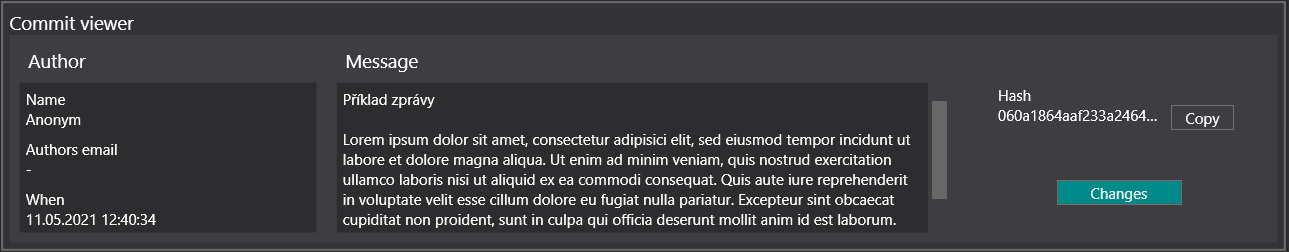
\includegraphics[width=1\linewidth]{commit-viewer.png}
   \caption{Verze pro revizi}

\vspace{5 mm}
\end{subfigure}
\begin{subfigure}[b]{13cm}
   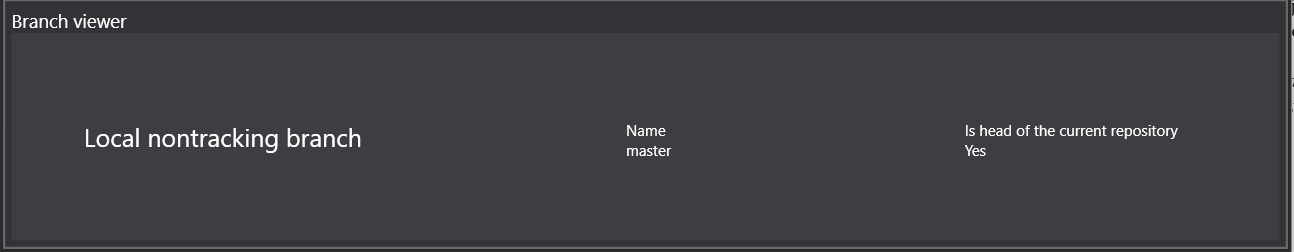
\includegraphics[width=1\linewidth]{branch-viewer.png}
   \caption{Verze pro větev}
\end{subfigure}
\caption{Panel s informacemi o zvoleném objektu grafu}
\label{fig:item-info}
\end{figure}

Každý uzel větve navíc může obsahovat ikony indikující, že je větev vzdálená, nebo že má připojenou některou vzdálenou větev. Panel s informacemi potom ukazuje o kolik verzí je daný uzel před/za sledovanou vzdálenou větví.

V grafu se lze pohybovat pomocí myši po stisknutí a podržení pravého tlačítka v oblasti grafu. Znázorňuje to i kurzor myši pro pohyb ve všech směrech. Celý graf lze pomocí kolečka myši nebo touchepadu zvětšovat a zmenšovat. Hranice pro posun se nachází několik centimetrů za nejkrajnějším objektem grafu.

V krajním případě lze na sebe nahromadit velké množství větví. Tento příklad v praxi nenastává, ale je možný. V takovém případě je výsledek nejen vizuálně ne příliš hezký, ale také je potom možné graf po celé délce posunovat zbytečně vysoko a navíc se kvůli velkému počtu grafických prvků na jednom místě může zhoršovat plynulost posunování v grafu. Do budoucna je proto počítáno s úspornějším řešením. Například zobrazit pouze jeden uzel a tlačítko pro výčet ostatních.

Koncept příkazu \kiinlinecode{text}{;}{git log} je v programu GitGUI nahrazen samotným grafem, který zrcadlí historii. Ve větších projektech ale může být obtížné vyhledávat konkrétní revize či větve pouze procházením grafu. Proto je v pravém horním rohu plochy pro zobrazení grafu přístupný nástroj pro vyhledávání \ref{fig:searchtool} (ukázka je provedena na projektu \cite{libgitreference}

\pic{10cm}{searchbar.png}{Ukázka vyhledávání}{searchtool}

Nástroj obsahuje pole pro vložení hledaného výrazu a vyskakovací našeptávač. Kromě toho také obsahuje tlačítko speciálně pro nalezení hlavy repozitáře. Našeptávač se zobrazí v případě, že byl upraven vyhledávací výraz, jeho délka je nenulová a některé položky grafu vyhledávání vyhovují. Přejít na hledanou položku v grafu je možné pouze výběrem (myší, nebo klávesnicí) v našeptávači. Tím se otevře panel s informacemi o položce a graf se posune hledanou položkou do zorného pole. Našeptávač je rozdělen do tří kategorií. Každá z těchto kategorií pak obsahuje nanejvýš tři návrhy, popřípadě není zobrazena neexistuje-li pro hledaný výraz žádný návrh. Kategorie jsou popořadě: Revize podle prvního řádku zprávy, větve podle názvu a revize podle jejich hash kódů. Nutno dodat, že se vyhledávané hodnoty porovnávají pouze od začátku.

\subsection{Uživatelé}
Současně s verzemi se v gitu ukládají i informace o autorovi, konkrétně jméno a e-mailová adresa. V programu GitGUI se automaticky použije výchozí uživatel se jménem \uv{Anonym} a adresou \uv{-}. Tento výchozí uživatel nelze smazat ani upravit. Je však možné dle libosti mazat, upravovat a vytvářet další uživatele. Slouží k tomu rozbalovací nabídka v pravém horním rohu okna \ref{fig:users}.

\pic{10cm}{users.png}{Nabídka uživatelů}{users}

Jak je na obrázku vidět, nabídka se skládá ze seznamu uživatelů (který po překročení určité velikosti stane rolovatelný) a tlačítek pro vytvoření nového uživatele a sdílení nebo aktualizaci databáze uživatelů.

Každý uživatel může kromě, z gitu známého, jména a adresy obsahovat ještě profilový obrázek. Výběrem tlačítka na pravé straně nevýchozího uživatele lze uživatele upravit, nebo smazat. Uživatel je vytvářen/upravován v samostatném okně. Výběr obrázku je nepovinný, ale jméno a adresa musí být validní. Pokud nejsou zadané hodnoty přípustné, u daného řádku je symbol červeného křížku a tlačítko pro potvrzení není povoleno, v opačném případě se objeví symbol zelené fajfky.

Požadavky pro hodnoty jsou:
\begin{description}
\item[Pro jméno:] neprázdný řetězec obsahující alespoň jeden znak, který není bílý.
\item[Pro adresu:] správný tvar e-mailové adresy.
\end{description}

Všechny revize, které mají autora, jenž je známý, a má přidělený profilový obrázek, mají jeho miniaturu umístěnou v levé části uzlu \ref{fig:user}.

\pic{10cm}{user.png}{Revize s obrázkem autora}{user}

Databázi uživatelů lze také sdílet. Po zvolení této možnosti se program dotáže na umístění, do kterého zkopíruje složku s daty o uživatelích. Opačně lze z takto sdílené složky aktualizovat databázi programu.

\subsection{Vytváření revizí}
Stisknutím tlačítka {\it Commit} se otevře nová karta. Je-l již karta pro vytvoření nové revize otevřena, nevytvoří se nová, ale přepne se na stávající.

Karta se dělí na tři hlavní části: adresář změn, okno pro detail změny a oblast pro specifikaci zprávy revize.

\subsubsection{Adresář změn}
Nachází se v levé části karty. Adresář tvoří stromovou strukturu. V listových uzlech stromu se nachází soubory, které byly změněny. V nelistových pak rodičovské složky až ke kořenové cestě, odpovídající uzel se nazývá {\it All}.

Každý listový uzel lze vybrat a tím zobrazit v pravé části karty detail změny. Většinou se jedná o jednoduchou textovou informaci, jako například: \uv{Nový soubor}, \uv{Smazaný soubor}, \uv{Přejmenovaný soubor}, \uv{změna je binární}. V případě textové změny je však zobrazen gitový \uv{diff}, neboli rozdíl současné verze od předchozí.

Každý uzel stromu také obsahuje zaškrtávací políčko. Zaškrtnuté změny se projeví v revizi, stejně jako kdyby se v příkazovém řádku přidaly do indexu pomocí příkazu \kiinlinecode{text}{;}{git add}. Ve výchozím stavu jsou všechny změny aktivní, to platí jak pro nově vytvořenou kartu, tak po jakékoliv změně v repozitáři.

\subsubsection{Detail změny}
Jak již bylo uvedeno, jediným zajímavým obsahem této oblasti je zobrazení souborového rozdílu. Postupně jsou pod sebou vypsané skývy ({\it hunk}) kódu obsahující změnu. Ty mají stejnou hlavičku, jako ve výsledku volání \kiinlinecode{text}{;}{git diff}. Obsah změny je ale formátován přehledněji a je barevně odlišená stará verze nová verze a nezměněná část.

\subsubsection{Zpráva}
Poslední částí je pole pro zprávu revize s tlačítkem potvrzení. Tlačítko je aktivní pouze když je vybrána alespoň jedna změna a text zprávy je neprázdný.

\pic{10cm}{create-commit.png}{Výřez karty vytvoření revize}{}

\subsection{Práce s větvemi}
Operace \kiinlinecode{text}{;}{git checkout} lze v GitGUI provést výběrem požadované větve, nebo revize v grafu a stisknutím tlačítka {\it Checkout}, to je aktivní právě když je některý uzel vybrán.

Kromě vytváření nových větví je potřeba je slučovat. Tato operace se provádí přímo v grafu stylem přetáhnutí uzlu jedné větve na druhou. Tím se vyvolá kontextová nabídka s výběrem požadované operace, a to buď Merge, anebo Rebase.

Při přetahování uzlu může nastat situace, kdy se slučovaná větev nenachází v aktuálním zorném poli. Jedna vlastnost, která toto řeší je možností oddalovat a přibližovat graf během přesunování. Tou druhou je automatické odsunování plátna grafu

 



 




\subsection{Algoritmus rozmístění uzlů v grafu}
\label{subsec:algorithm}














%% Závěry práce. V jazyce práce a anglicky. Text pro jiný než
%% nastavený jazyk práce (nepovinným parametrem language makra
%% \documentclass, výchozí český) se zadává použitím makra s uvedením
%% jazyka jako nepovinného parametru.
\begin{kiconclusions}
Závěr práce v \uv{českém} jazyce.
\end{kiconclusions}

\begin{kiconclusions}[english]
Thesis conclusions in \uv{English}.
\end{kiconclusions}

%% Přílohy obsahu textu práce, za makrem \appendix.
\appendix

%% Obsah přiloženého CD/DVD. Poslední příloha. Upravte podle vlastní
%% práce!
\section{Obsah přiloženého CD/DVD} \label{sec:ObsahCD}

\begin{description}

\item[\texttt{bin/}] \hfill \\
  Instalátor

\end{description}

Navíc CD/DVD obsahuje:

\begin{description}

\item[\texttt{literature/}] \hfill \\
  Vybrané položky bibliografie, příp.~jiná užitečná literatura
  vztahující se k~práci.

\end{description}

%% -------------------------------------------------------------------

%% Sazba volitelného seznamu zkratek, za přílohami.
\printglossary

%% Sazba povinné bibliografie, za přílohami (případně i za seznamem
%% zkratek). Při použití BibLaTeXu použijte makro
%% \printbibliography. jinak prostředí thebibliography. Ne obojí!

%% Sazba i v textu necitovaných zdrojů, při použití
%% BibLaTeXu. Volitelné.
\nocite{*}
%% Vlastní sazba bibliografie při použití BibLaTeXu.
\printbibliography

%% Bibliografie, včetně sazby, při nepoužití BibLaTeXu.
% \begin{thebibliography}{9}
%\bibitem{kniha2} \uppercase{Hawke}, Paul. NanoHttpd: Light-weight HTTP server designed for embedding in other applications. GitHub [online]. 2014-05-12. [cit. 2014-12-06]. Dostupné z: \url{https://github.com/NanoHttpd/nanohttpd}
%
%\bibitem{jeske13} \uppercase{Jeske}, David; \uppercase{Novák}, Josef. Simple HTTP Server in \csharp: Threaded synchronous HTTP Server abstract class, to respond to HTTP requests. CodeProject: For those who code [online]. 2014-05-24. [cit. 2014-12-06]. Dostupné z: \url{http://www.codeproject.com/Articles/137979/Simple-HTTP-Server-in-C}
%
%\bibitem{uzis2012} \uppercase{ÚSTAV ZDRAVOTNICKÝCH INFORMACÍ A STATISTIKY ČR}. Lékaři, zubní lékaři a farmaceuti 2012 [online]. Praha 2, Palackého náměstí 4: Ústav zdravotnických informací a statistiky ČR, 2012 [cit. 2014-12-06]. ISBN 978-80-7472-089-5. Dostupné z: \url{http://www.uzis.cz/publikace/lekari-zubni-lekari-farmaceuti-2012}
% \end{thebibliography}

%% Sazba volitelného rejstříku, za bibliografií.
\printindex

\end{document}
